\chapter{Modelo de datos}
\label{cap:modeloDeDatos}
En este capítulo se explicará todo el modelo de datos de la aplicación. En primer lugar, se hará una descripición de todas las estructuras de datos utilizadas, explicándolas brevemente para dar un poco de contexto, sin embargo, siempre se recomienda ver y tocar el código para entenderlo en profundidad. En segundo lugar se explicarán todos los servicios utilizados para mantener la persistencia: Firebase (principal herramienta utilizada como base de datos remota), Datastore (se ha utilizado para guardar en local preferencias del sistema) y por último se explicará como se ha utilizado el patrón Singleton para evitar tener que usar una base de datos local como \href{https://developer.android.com/training/data-storage/room/}{Room}, logrando así una aplicación completa que pueda interactuar con otros dispositivos a través de la red.
\section{Descripción del modelo de datos}
\begin{itemize}
    \item \textbf{ActorModel}: es la estructura de datos que almacena todos los datos de usuario, se usa la misma tanto para usuarios como para profesionales ya que admite campos nulos para aquellos atributos que solo corresponden a un tipo de actor, en esta estructura se guarda también el tipo de actor, la lista de favoritos (lista con otros \textit{ActorModel}), la calificación y el número de calificaciones.
    \begin{figure}[h]
        \centering
        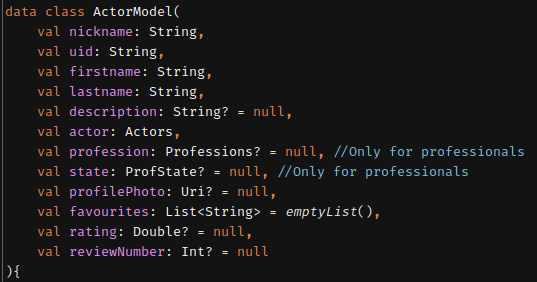
\includegraphics[width = 0.7\textwidth]{Imagenes/Fuentes/actorModel.png}
        \caption{Clase ActorModel.}
        \label{fig:actorModel}
    \end{figure}
    \item \textbf{ServiceModel}: guarda el modelo de un servicio, cuenta con distintos campos como la categoría del servicio, si está activo o no, y el propietario del servicio (un \textit{ActorModel}).
    \begin{figure}[h]
        \centering
        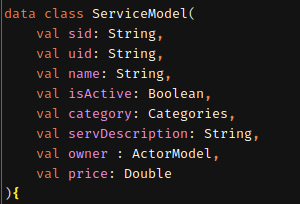
\includegraphics[width = 0.5\textwidth]{Imagenes/Fuentes/ServiceModel.png}
        \caption{Clase ServiceModel.}
        \label{fig:ServiceModel}
    \end{figure}
    \item \textbf{JobModel}: esta clase guarda tanto solicitudes de trabajo como trabajos activos, en un principio se hicieron dos clases separadas para esto, pero se comprobó que la funcionalidad era la misma y se unificó en una sola clase para evitar duplicaciones de código, relacionan el profesional, el usuario y el servicio.
    \begin{figure}[h]
        \centering
        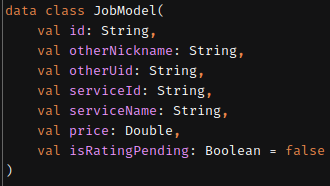
\includegraphics[width = 0.5\textwidth]{Imagenes/Fuentes/JobModel.png}
        \caption{Clase JobModel.}
        \label{fig:JobModel}
    \end{figure}
    \item \textbf{ChatListItemModel}: representa un item en la lista de chats recientes, guarda solo los campos necesarios para mostrar al usuario sin tener que volver a acceder a base de datos para sacar el \textit{ActorModel} completo.
    \begin{figure}[h]
        \centering
        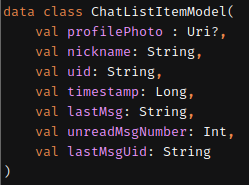
\includegraphics[width = 0.3\textwidth]{Imagenes/Fuentes/ChatListItemModel.png}
        \caption{Clase ChatListItemModel.}
        \label{fig:ChatListItemModel}
    \end{figure}
    \item \textbf{ChatMsgModel}: esta clase representa un mensaje en el chat, guarda el contenido del mensaje, un \textit{timestamp} para saber el momento exacto en el que se envió de cara a ordenarlo en la lista de mensajes, así como para mostrarle la hora al usuario y si el usuario es propietario (lo ha enviado él) o no (lo ha recibido) del mensaje.
    \begin{figure}[h]
        \centering
        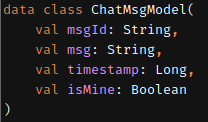
\includegraphics[width = 0.4\textwidth]{Imagenes/Fuentes/ChatMsgModel.png}
        \caption{Clase ChatMsgModel.}
        \label{fig:ChatMsgModel}
    \end{figure}
    \item \textbf{LocationModel}: representa la localización de un usuario, solo guarda los campos que es necesario mostrar en el mapa, la localización y el id del usuario (para poder extraer sus datos si fuera necesario).
    \begin{figure}[h]
        \centering
        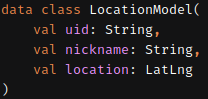
\includegraphics[width = 0.4\textwidth]{Imagenes/Fuentes/LocationModel.png}
        \caption{Clase LocationModel.}
        \label{fig:LocationModel}
    \end{figure}
    \item \textbf{Enums}: También se han guardado una serie de enumerados para guardar cosas como los tipos de actores, las categorías de servicios, profesiones, etc. Esto hace que sea muy sencillo añadir nuevos en caso de necesidad sin tener que cambiar código existente, solo añadir nuevo (\textit{Open/Closed Principle}, véase el apartado \ref{subsec:solid}).
    \begin{figure}[h]
        \centering
        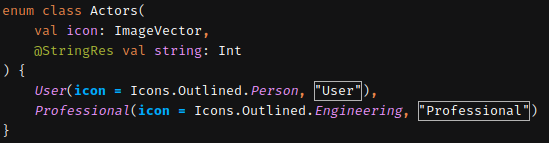
\includegraphics[width = 0.7\textwidth]{Imagenes/Fuentes/ejemplo_enum.png}
        \caption{Ejemplo de enumerado (actores).}
        \label{fig:ejemplo_enum}
    \end{figure}
\end{itemize}

\hypertarget{subsec:firebase}{}
\section{Firebase} 
\label{subsec:firebase}
\href{https://firebase.google.com/}{Firebase} es una plataforma web desarrollada por Google que ofrece una amplia gama de servicios para ayudar a los desarrolladores a crear y mejorar aplicaciones. En Profinder, se ha utilizado como \textit{backend} para toda la aplicación y ha aportado la capacidad de plasmar el modelo de datos de la aplicación a una base datos, así como autenticación y almacenamiento para fotos. A continuación se ha explicado cada servicio utilizado.
\subsection{Authentication}
\href{https://firebase.google.com/docs/auth/}{Firebase Authentication} es un servicio de autenticación que ahorra todo el proceso de gurdado y cifrado de cotraseñas, también gestiona las sesiones de cada usuario, permitiendo mantener la sesión iniciada.Tiene compatibilidad para configurar diversos métodos de autenticación, sin embargo, en esta aplicación solo se ha considerado oportuno implementar la autenticación con \textit{email} y contraseña aunque si se quisiera sería sencillo añadir otros métodos.
\begin{figure}[h]
    \centering
    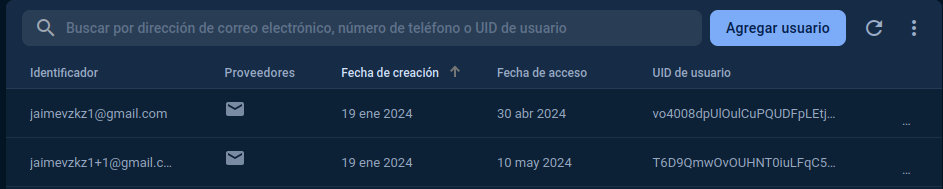
\includegraphics[width = 1\textwidth]{Imagenes/Fuentes/ejemplo_auth.png}
    \caption{Captura de pantalla del panel de control de Firebase Authentication.}
    \label{fig:ejemplo_auth}
\end{figure}
\hypertarget{subsec:firestore}{}
\subsection{Firestore} 
\href{https://firebase.google.com/docs/firestore/}{Firebase Firestore} ha sido la principal base de datos del proyecto, es de tipo no SQL lo cual ha presentado algunas ventajas pero también muchos desafios ya que en este tipo de bases de datos es muy fácil caer en la duplicación de datos y ha sido necesario gastar mucho tiempo en pensar la mejor forma de implementarla. 

Esta base de datos ha sido dividida en tres colecciones explicadas a continuación (véase el apéndice \ref{Appendix:bd_design} con el diagrama del diseño):
\begin{itemize}
    \item \textbf{users}: cada documento de esta colección se guarda con un id generado automáticamente y es donde se almacenan los datos de cada usuario, así como los \textit{jobs} y \textit{requests}.
    \item \textbf{services}: cada documento de esta colección se guardaba con un id generado automáticamente y es donde se almacenaban los datos de cada servicio.
    \item \textbf{locations}: cada elemento de esta colección representa la localización de un usuario, se generan con una id igual a la id del usuario y guardan el \textit{nickname} del usuario a parte de su localización
\end{itemize}
\begin{figure}[h]
    \centering
    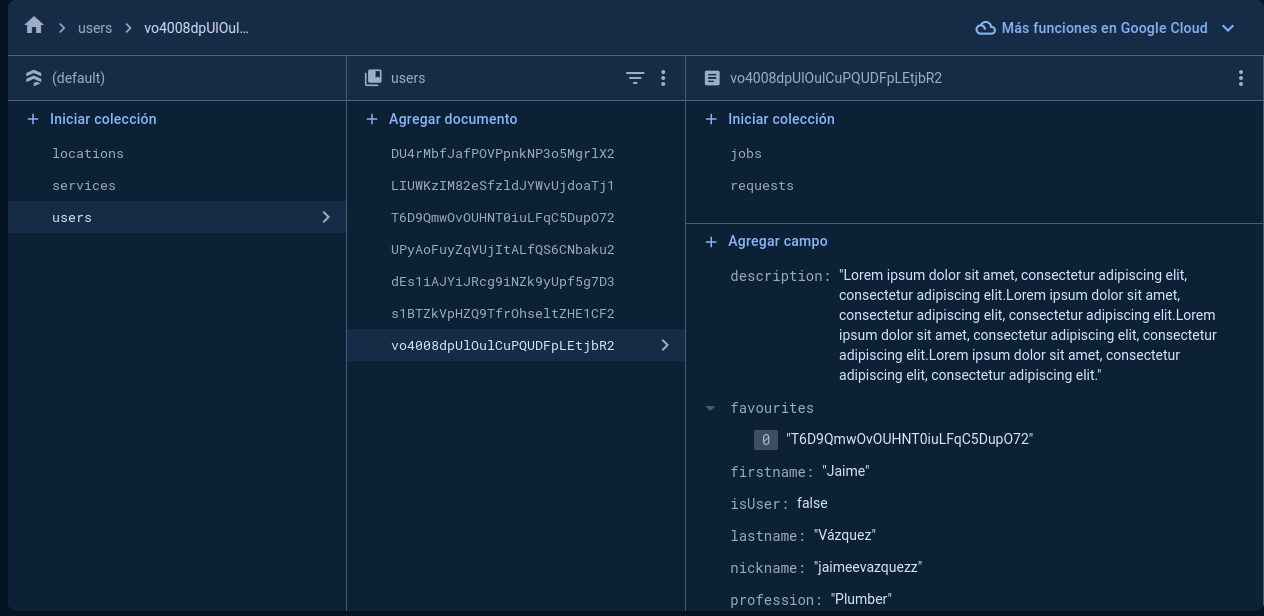
\includegraphics[width = 1\textwidth]{Imagenes/Fuentes/ejemplo_firestore.png}
    \caption{Captura de pantalla del panel de control de la base de datos Firestore.}
    \label{fig:ejemplo_firestore}
\end{figure}
\hypertarget{subsec:realtime}{}
\subsection{Realtime Database}
\href{https://firebase.google.com/docs/database/}{Realtime database} es una base datos de baja latencia, menos sofisticada que \hyperlink{subsec:firestore}{Firestore} pero cuyas funcionalidades han encajado perfectamente con las necesidades del proyecto. Se ha utilizado para toda la funcionalidad de chat ya que al ser los mensajes en tiempo real, era necesario que la latencia fuera mínima. 

En Realtime, los datos se guardan en formato JSON (\textit{JavaScript Object Notation}). En esta aplicación se ha divido en la lista de chats recientes (conteniendo atributos como el último mensaje, los participantes, la hora y el número de mensajes sin leer por cada conversación entre dos actores de la aplicación) y los chats en sí (conteniendo cada mensaje de una conversación con la hora en que fue mandado).
\begin{figure}[h]
    \centering
    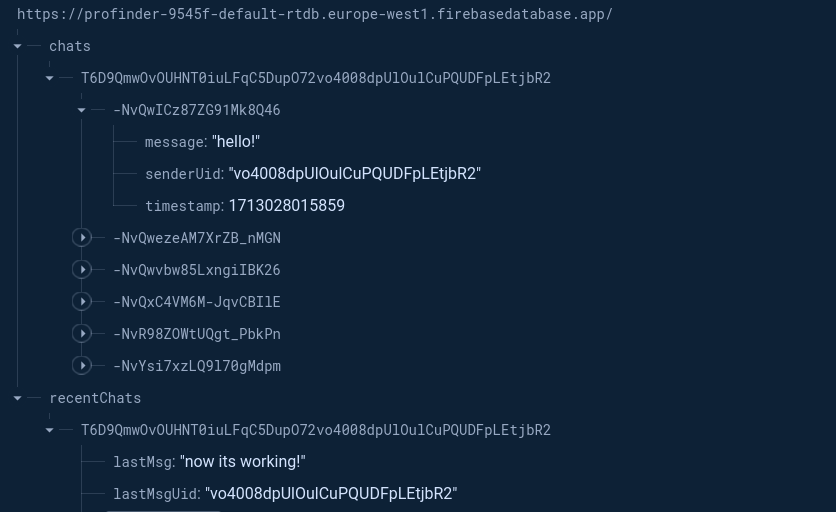
\includegraphics[width = 0.8\textwidth]{Imagenes/Fuentes/ejemplo_realtime.png}
    \caption{Captura de pantalla de la estruectura de Realtime Database}
    \label{fig:ejemplo_realtime}
\end{figure}
\subsection{Storage}
\href{https://firebase.google.com/docs/storage/}{Firebase storage} es un servicio de alamcenamiento en la nube. Se ha utilizado para almacenar las fotos de perfil de los actores de la aplicacion. Cada foto de perfil se guarda en una carpeta cuyo nombre es el id del actor y se accede a ella a traves de una uri autogenerada que se procesa en la aplicación usando \hyperlink{subsec:coil}{Coil}.
\section{Datastore}
\href{https://developer.android.com/topic/libraries/architecture/datastore}{Data store} es un sistema de almacenamiento persistente que permite guardar pares clave valor en la aplicación para un acceso rápido a través de \href{https://developer.android.com/kotlin/coroutines}{corrutinas}. 
En el caso de Profinder se ha utilizado para guardar 2 cosas:
\begin{itemize}
    \item \textbf{Tema de la aplicación}: de tal forma que cuando se cambia su valor, devuelve un \href{https://developer.android.com/kotlin/flow}{\textit{flow}} que indica a la Main Activity el tema que debe utilizar. Este tema se mantiene en caché por lo que se podría cerrar la aplicación y al abrirla se recordaría el tema establecido.
    \item \textbf{El id del usuario iniciado}: De tal forma que cuando se se necesiten datos del usuario desde cualquier parte de la app se puede conseguir el id (que es único en base de datos) según necesidad, esto servirá para un acceso más rápido en Firestore debido a que es una base de datos que se indexa con este campo.
\end{itemize}

\section{Uso del patrón Singleton como modelo de persistencia}
En la programación Android, la persistencia de datos es muy importante ya que al contrario que en otro tipo de programas, cada poco tiempo se borran todos los datos no persistidos para evitar que la aplicación ocupe demasiado espacio en el dispositivo. En este contexto es donde se presenta el problema.

A lo largo del desarrollo de otras aplicaciones (en preparación a esta) se encontró que el uso de una base de datos local suponía una carga de espacio en la aplicación y en tiempo de compilación que la ralentizaba, más allá de esto, las necesidades de Profinder implicaban que los datos fueran actualizados cada no demasiado tiempo puesto que tanto servicios; como favoritos; como los datos de usuario están diseñados para cambiar con frecuencia entre los distintos actores de la aplicación. Por estos motivos se decidió buscar un sistema alternativo que se adecuara a las necesidades de la aplicación: actualización frecuente y poca carga en memoria sin tener que estar accediendo constantemente al servicio remoto (\hyperlink{subsec:firestore}{Firestore}) ya que esto supondría un coste económico.

Esta solución se ha implementado siguiendo el patrón \textit{Singleton}. Los datos a persistir almacenan en una clase que los guarda de la siguiente forma: si los datos están cacheados los devuelve, si no, los saca del servicio remoto, los cachea y los devuelve. De esta forma la próxima vez que se accedan los datos, estarán cacheados y no hará falta llamar al servicio remoto.
\begin{figure}[h]
    \centering
    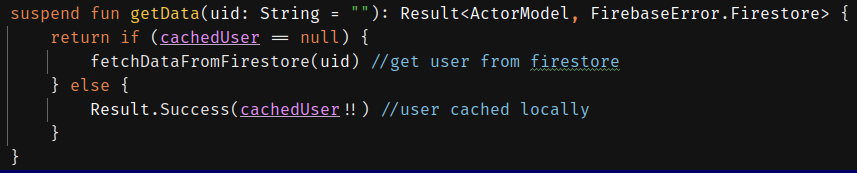
\includegraphics[width = 1\textwidth]{Imagenes/Fuentes/ejemplo_singleton1.png}
    \caption{Ejemplo de función getData()}
    \label{fig:ejemplo_singleton1}
\end{figure}

Para acceder a esta función es donde creamos el Singleton que será accedido desde cualquier lugar donde se necesiten los datos:
\begin{figure}[h]
    \centering
    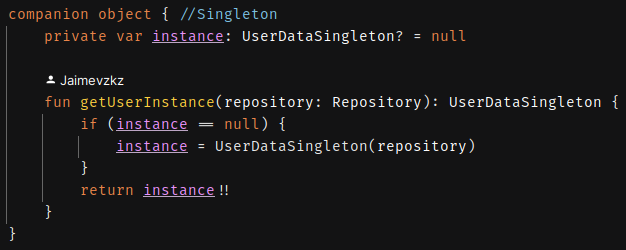
\includegraphics[width = 1\textwidth]{Imagenes/Fuentes/ejemplo_singleton2.png}
    \caption{Ejemplo de Singleton con datos de usuario}
    \label{fig:ejemplo_singleton2}
\end{figure}